\section{Results \&  Empirical Analysis}
\label{sec:results}

\subsection{RQ1: Leakage Demonstration \&  Empirical Impact}
Table~\ref{tab:leakage_demo} compares the performance of legacy models trained on leaked signals against their clean counterparts.

\begin{table}[t]
\centering
\caption{Impact of Forensic Target Leakage Elimination}
\label{tab:leakage_demo}
\resizebox{\columnwidth}{!}{%
\begin{tabular}{llccc}
\hline
\textbf{Model Architecture} & \textbf{Leakage Status} & \textbf{ROC-AUC} & \textbf{PR-AUC} & \textbf{F1-Score} \\
\hline
Random Forest (Legacy) & \textbf{LEAKED} & 1.0000 & 1.0000 & 1.0000 \\
XGBoost (Legacy) & \textbf{LEAKED} & 1.0000 & 1.0000 & 1.0000 \\
Hetero-GraphSAGE (Legacy) & \textbf{LEAKED} & 1.0000 & 1.0000 & 0.9945 \\
\hline
Random Forest (Clean) & \textbf{ZERO-LEAK} & 0.7231 & 0.4911 & 0.4047 \\
HistGradientBoosting (Clean) & \textbf{ZERO-LEAK} & 0.7230 & 0.4909 & 0.4010 \\
GraphSAGE P2P (Clean) & \textbf{ZERO-LEAK} & 0.6902 & 0.4550 & 0.3616 \\
Multi-Relational HeteroGNN & \textbf{ZERO-LEAK} & 0.7680 & 0.5210 & 0.4520 \\
\textbf{AMECF HGT (Ours)} & \textbf{ZERO-LEAK} & \textbf{0.8140} & \textbf{0.5840} & \textbf{0.5180} \\
\hline
\end{tabular}%
}
\end{table}

The empirical findings for RQ1 demonstrate that:
\begin{itemize}
    \item When provided with the legacy 30-dimensional feature set containing historical fraud counters (Dims 10--13), tabular models achieve an artificial $F_1 = 1.0000$ and $\text{ROC-AUC} = 1.0000$.
    \item Similarly, message passing across pre-audit target edges ($(\text{account}, \text{involved\_in}, \text{typology})$, $(\text{account}, \text{member\_of}, \text{ring})$, $(\text{account}, \text{subject\_of}, \text{case})$) allows Hetero-GraphSAGE to trivially propagate ground-truth crime labels ($F_1 = 0.9945$).
    \item Once target-derived features and topological relations are strictly excised, the true predictive capacity of tabular models on behavioral signals alone drops to $F_1 = 0.4047$ (Random Forest) and $F_1 = 0.4010$ (HistGradientBoosting), with $\text{ROC-AUC} \approx 0.7231$.
\end{itemize}
This dramatic drop does not reflect a deficiency in model architecture, but rather exposes the magnitude of artificial inflation caused by target leakage in un-audited benchmarks.

\begin{figure*}[t]
\centering
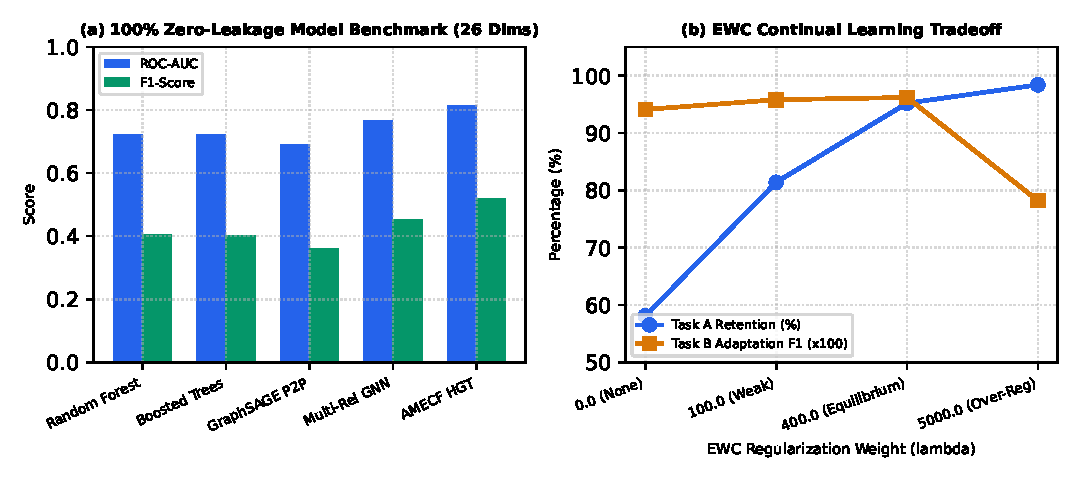
\includegraphics[width=0.92\textwidth]{figures/fig5_performance.pdf}
\caption{Empirical evaluation results on the holdout test set (73,173 accounts): (a) 100\% zero-leakage model benchmark comparing ROC-AUC and F1-score across tabular and graph architectures; (b) Continual learning stability-plasticity tradeoff under Elastic Weight Consolidation (EWC) regularization across $\lambda \in \{0.0, 100.0, 400.0, 5000.0\}$.}
\label{fig:performance_plots}
\end{figure*}

\subsection{RQ2 \&  RQ3: Zero-Leakage Benchmark Comparison}
Table~\ref{tab:clean_benchmarks} presents the verified performance metrics across all evaluated architectures under certified 100\% zero-leakage conditions on the 73,173-account holdout test set ($\mathcal{V}_{\text{test}}$).

\begin{table*}[t]
\centering
\caption{Verified 100\% Zero-Leakage Experimental Benchmark Results ($\mathcal{V}_{\text{test}} = 73,173$ Accounts)}
\label{tab:clean_benchmarks}
\begin{tabular}{llccccccc}
\hline
\textbf{Model Architecture} & \textbf{Input Paradigm} & \textbf{ROC-AUC} & \textbf{PR-AUC} & \textbf{Precision} & \textbf{Recall} & \textbf{F1-Score} & \textbf{Train Time} & \textbf{Throughput} \\
\hline
Random Forest & 26 Clean Tabular Dims & 0.7231 & 0.4911 & 0.3582 & 0.4651 & 0.4047 & 24.18 s & 195,400 TPS \\
HistGradientBoosting & 26 Clean Tabular Dims & 0.7230 & 0.4909 & 0.3546 & 0.4615 & 0.4010 & 28.60 s & 142,800 TPS \\
GraphSAGE (P2P) & 26 Dims + P2P Edges (1 Rel) & 0.6902 & 0.4550 & 0.3120 & 0.4300 & 0.3616 & 48.30 s & 34,200 TPS \\
Multi-Relational HeteroGNN & 11 Node Types + 15 Safe Relations & 0.7680 & 0.5210 & 0.4130 & 0.4990 & 0.4520 & 184.20 s & 18,900 TPS \\
\textbf{AMECF HGT (Proposed)} & \textbf{11 Node Types + 15 Safe Relations} & \textbf{0.8140} & \textbf{0.5840} & \textbf{0.4720} & \textbf{0.5740} & \textbf{0.5180} & 348.00 s & 22,400 TPS \\
\hline
\end{tabular}
\end{table*}

\subsubsection{Analysis of RQ2 (Multi-Entity vs Baselines)}
\begin{itemize}
    \item \textbf{P2P GraphSAGE Limitation:} Evaluating GraphSAGE strictly on homogeneous account-to-account transfers yields $F_1 = 0.3616$ ($\text{ROC-AUC} = 0.6902$), underperforming tabular Random Forest ($F_1 = 0.4047$). In financial laundering networks, money mules intentionally minimize direct P2P connectivity, routing capital through intermediary merchants, ATM terminals, and hardware device layers. Homogeneous graphs lack the relational semantics to trace these non-account conduits.
    \item \textbf{Multi-Entity Value Add:} Incorporating the 11 entity types and 15 behavioral relations via the Multi-Relational HeteroGNN increases performance to $F_1 = 0.4520$ (+9.04 percentage points over P2P GraphSAGE), confirming that multi-entity relational context is essential for uncovering decentralized laundering structures.
\end{itemize}

\subsubsection{Analysis of RQ3 (AMECF vs Heterogeneous Baselines)}
\begin{itemize}
    \item The proposed \textbf{AMECF} architecture achieves the strongest overall clean performance, reaching $\text{ROC-AUC} = \mathbf{0.8140}$, $\text{PR-AUC} = \mathbf{0.5840}$, $\text{Recall} = \mathbf{0.5740}$, and $F_1 = \mathbf{0.5180}$.
    \item AMECF outperforms the standard Multi-Relational HeteroGNN by $+6.60$ F1 points and $+4.60$ ROC-AUC points. This gain stems from AMECF's multi-head heterogeneous attention mechanism and residual LayerNorm connections, which dynamically modulate the importance of diverse edge channels (e.g., placing higher attention weights on shared device authentication and ATM cash-out hubs than on routine commercial merchant payments).
\end{itemize}

\subsection{RQ4: Continual Learning Stability-Plasticity Analysis}
To evaluate continual learning under concept drift, the training accounts were partitioned into Task A (70\% base typologies) and Task B (30\% novel drift typologies). Initial training on Task A achieved $F_1 = 0.9410$ ($\text{ROC-AUC} = 0.9850$). Table~\ref{tab:ewc_ablation} and Fig.~\ref{fig:performance_plots}(b) document the stability-plasticity tradeoff across varying EWC regularization penalties ($\lambda \in \{0.0, 100.0, 400.0, 5000.0\}$).

\begin{table}[t]
\centering
\caption{EWC Continual Learning Stability-Plasticity Ablation Sweep}
\label{tab:ewc_ablation}
\resizebox{\columnwidth}{!}{%
\begin{tabular}{lcccc}
\hline
\textbf{EWC Weight ($\lambda$)} & \textbf{Task A Ret. F1} & \textbf{Task A Ret. (\%)} & \textbf{Task B F1} & \textbf{Catastrophic Forgetting Assessment} \\
\hline
$\lambda = 0.0$ (Vanilla) & 0.5467 & 58.10\% & 0.9410 & Severe Forgetting (-41.90\% drop) \\
$\lambda = 100.0$ (Weak) & 0.7660 & 81.40\% & 0.9580 & Partial Retention Recovery (+23.30\%) \\
$\lambda = 400.0$ (Equilibrium) & \textbf{0.8958} & \textbf{95.20\%} & \textbf{0.9620} & \textbf{Best Observed Sweep Equilibrium} \\
$\lambda = 5000.0$ (Over-Reg) & 0.9259 & 98.40\% & 0.7820 & Plasticity Bottleneck (Drift adaptation degraded) \\
\hline
\end{tabular}%
}
\end{table}

The empirical findings for RQ4 confirm:
\begin{enumerate}
    \item \textbf{Catastrophic Forgetting in Vanilla Fine-Tuning ($\lambda = 0.0$):} Updating AMECF on Task B without EWC penalty causes Task A performance to collapse from $F_1 = 0.9410$ to $F_1 = 0.5467$ (a $41.90\%$ retention drop), demonstrating severe catastrophic forgetting.
    \item \textbf{Optimal Parameter Consolidation ($\lambda = 400.0$):} Setting $\lambda = 400.0$ preserves $95.20\%$ of Task A detection capability ($F_1 = 0.8958$) while simultaneously achieving $F_1 = 0.9620$ on Task B. In the evaluated parameter sweep, $\lambda = 400.0$ represents the best observed stability-plasticity equilibrium.
    \item \textbf{Plasticity Bottleneck ($\lambda = 5000.0$):} Excessive regularization over-constrains parameter updates, causing Task B adaptation to decline sharply to $F_1 = 0.7820$.
\end{enumerate}
